\documentclass[10pt,a4paper]{letter}
\usepackage[utf8]{inputenc}

\usepackage{xeCJK}
\setCJKmainfont[BoldFont=SimHei,ItalicFont=SimSun]{SimHei}

\usepackage{amsmath}
\usepackage{amsfonts}
\usepackage{amssymb}
\usepackage{graphicx}
\usepackage{hyperref}

\setlength\topmargin{-70pt}
\setlength\textheight{10in}

\address{Yan King Yin, 7B Clear View, Discovery Bay, HK} 
% \signature{Yan King Yin}
\begin{document} 

\begin{letter}{Poly U Library: application for library card}


\includegraphics[scale=0.5]{genifer-logo-Stephenie-Marie.png}

\opening{Dear Poly U Library,} 
 
I am the founder of General Intelligence Research Group, a company focusing on R\&D of artificial intelligence technologies.

I have previously worked with:
\begin{itemize}
 \item  Dr Ben Goertzel (currently in Poly U Design School) 
 \item Dr 劉文印 (currently in City U department of computer science) 
\end{itemize}
in the AI field.

I created the open-source project Genifer:
\begin{itemize}
\item \hyperref[https://code.google.com/p/genifer/]{https://code.google.com/p/genifer/}
\item \hyperref[https://github.com/Cybernetic1/genifer5-c]{https://github.com/Cybernetic1/genifer5-c}
\end{itemize}

One of my published journal paper is:
\begin{itemize}
\item \textit{Fuzzy-Probabilistic Logic for Common Sense}. \textbf{AGI 2012:} 372-379
\end{itemize}

I have written a book on artificial general intelligence, published online:
\begin{itemize}
\item \hyperref[https://drive.google.com/file/d/0Bx3_S9SExak-TUc2aFVGZEk3QzQ]{https://drive.google.com/file/d/0Bx3\_S9SExak-TUc2aFVGZEk3QzQ}
\end{itemize}

I have also published numerous educational videos (related to artificial intelligence) on YouTube, such as:
\begin{itemize}
\item (P = NP problem) \hyperref[https://www.youtube.com/watch?v=9MwGPrQ8yKg]{https://www.youtube.com/watch?v=9MwGPrQ8yKg}
\item (Galois theory) \hyperref[https://www.youtube.com/watch?v=PO3MlDJjWrE]{https://www.youtube.com/watch?v=PO3MlDJjWrE}
\item (Neural networks) \hyperref[https://www.youtube.com/watch?v=Ow7Hc-xsweM]{https://www.youtube.com/watch?v=Ow7Hc-xsweM}
\item (Entropy) \hyperref[https://www.youtube.com/watch?v=faM2u1KadNI]{https://www.youtube.com/watch?v=faM2u1KadNI}
\end{itemize}

My research could result in commercial applications such as:  machine translation, question answering, and may have profound implications for future technologies.  I hope my company may one day benefit the Hong-Kong and global economy.

\closing{Yours sincerely,\\ Yan King Yin} 
%\cc{Cclist} 
%\ps{adding a postscript} 
%\encl{list of enclosed material} 

% 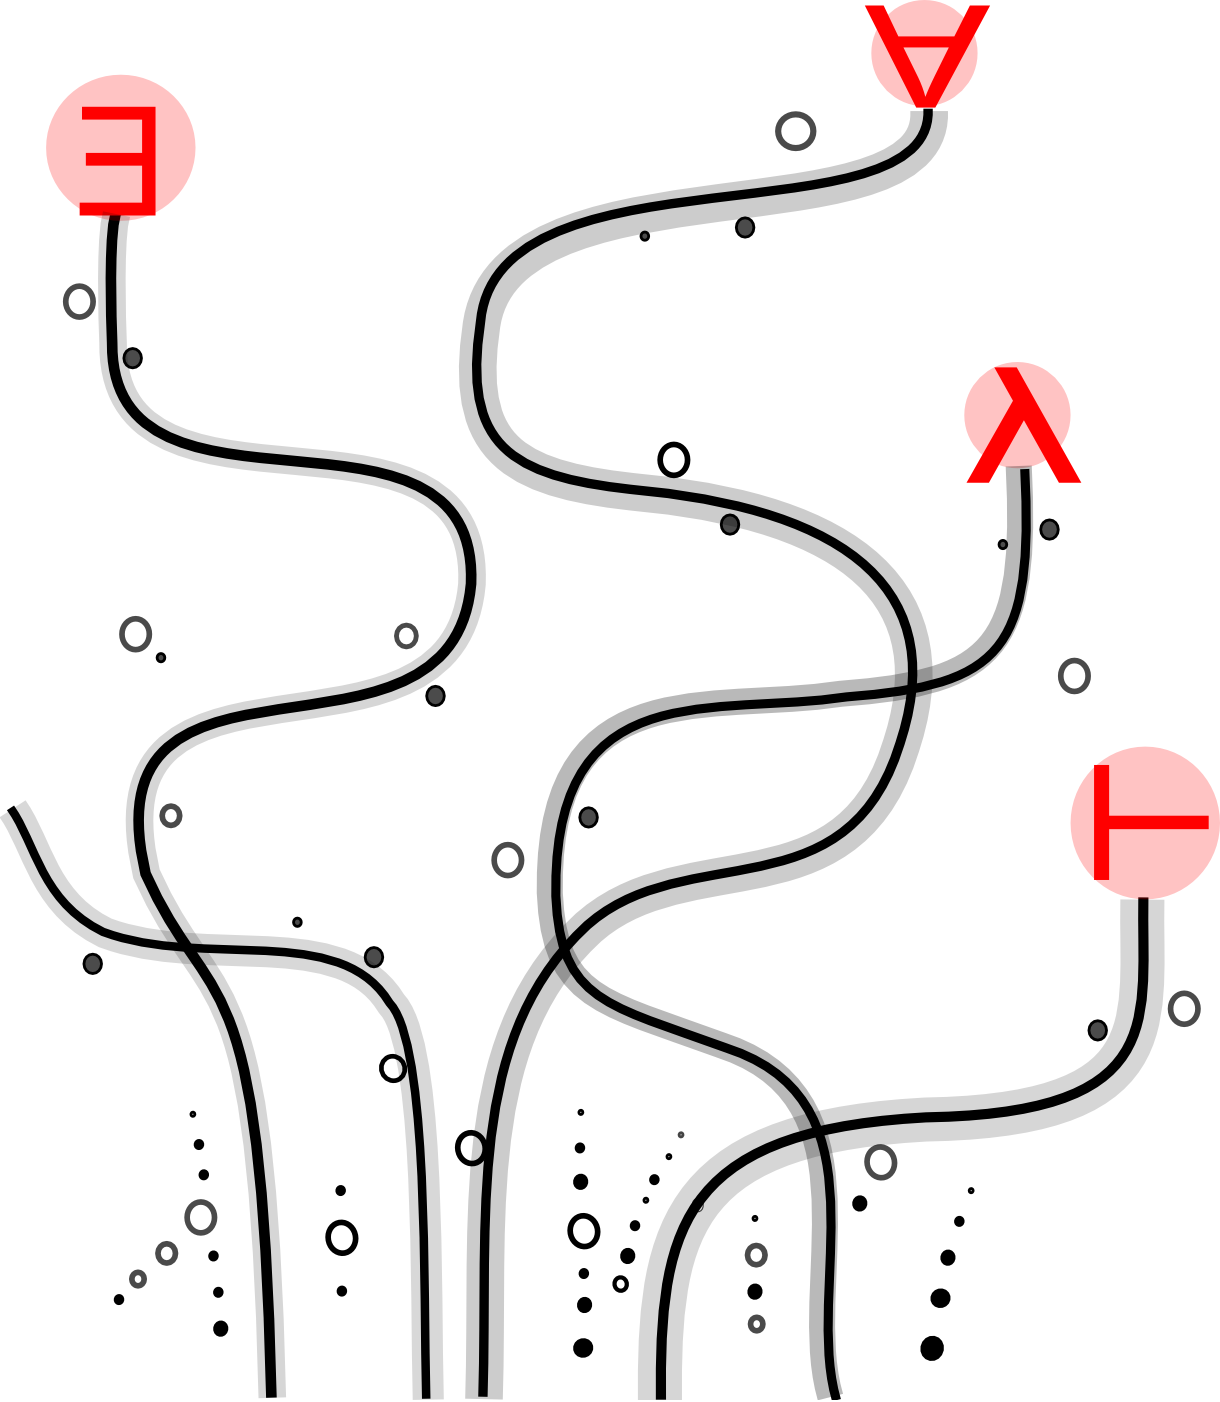
\includegraphics[scale=1.0]{Genifer-flowers.png}

\end{letter} 
\end{document}